% The preliminary material of your report should contain:
% \begin{itemize}
% \item
% The title page.
% \item
% An abstract page.
% \item
% Declaration of ethics and own work.
% \item
% Optionally an acknowledgements page.
% \item
% The table of contents.
% \end{itemize}

% As in this example \texttt{skeleton.tex}, the above material should be
% included between:
% \begin{verbatim}
% \begin{preliminary}
%     ...
% \end{preliminary}
% \end{verbatim}
% This style file uses roman numeral page numbers for the preliminary material.

% The main content of the dissertation, starting with the first chapter,
% starts with page~1. \emph{\textbf{The main content must not go beyond page~40.}}

% The report then contains a bibliography and any appendices, which may go beyond
% page~40. The appendices are only for any supporting material that's important to
% go on record. However, you cannot assume markers of dissertations will read them.

% You may not change the dissertation format (e.g., reduce the font size, change
% the margins, or reduce the line spacing from the default 1.5 spacing). Be
% careful if you copy-paste packages into your document preamble from elsewhere.
% Some \LaTeX{} packages, such as \texttt{fullpage} or \texttt{savetrees}, change
% the margins of your document. Do not include them!

% Over-length or incorrectly-formatted dissertations will not be accepted and you
% would have to modify your dissertation and resubmit. You cannot assume we will
% check your submission before the final deadline and if it requires resubmission
% after the deadline to conform to the page and style requirements you will be
% subject to the usual late penalties based on your final submission time.

% \section{Using Sections}

% Divide your chapters into sub-parts as appropriate.

% \section{Citations}

% Citations (such as \cite{P1} or \cite{P2}) can be generated using
% \texttt{BibTeX}. For more advanced usage, we recommend using the \texttt{natbib}
% package or the newer \texttt{biblatex} system.

% These examples use a numerical citation style. You may use any consistent
% reference style that you prefer, including ``(Author, Year)'' citations.


% objective, users, benefits, scope of work, relevant works, previous works, future works, project background, techniques


\section{Problem Statement and Its Significance}

% Business process management (BPM) tools are software that allow people with low to no background knowledge of coding to develop, automate, and manage business workflows by themselves. As a consequence, BPM tools provide key value to today's industrial companies because of a vast number of necessary repetitive tasks.
% Not only do BPM tools allow companies to develop workflows, but they also correct and prevent process logic by themselves.
% This helps the companies to only focus on the actual business logic in the tasks. Due to the lowering of the required knowledge barrier, this opens a number of opportunities for workflow creation.

% Business process management (BPM) tools are software to help manage, measure, and improve business processes through systematic workflows \cite{whatisbpm}.
% BPM tools are widely used by a vast number of companies across the world \cite{bpmcompanies} because they provide valuable things to companies, such as 

% BPM could be considered as: a customer‐focused approach to the systematic management, measurement and improvement of all company processes through cross‐functional teamwork and employee empowerment.
% The primary function of a BPM solution is to assist business analysts in modeling and optimizing the processes of their organization
%  \cite{bpmcompanies}
% BPM tools are convenient to a vast number of industrial companies.
% BPM tools require no prior coding experience to develop workflows and yet, are sufficiently customisable for more experienced users to build more complex workflows.

% Checklist here
% However, workflows do not contain only automated processes.
% they sometimes need human interaction
% but humans are dumb and prune to mistakes
% checklist is the answer because it guides humans through a pre-built list of items they need to do. this ensures both consistency and completeness of a certain task.

A workflow is a repeatable series of processes that transforms, provides, and computes information or services. 
Workflows are sometimes complicated and oftentimes require some form of inputs in order to proceed.
Inputs can come through multiple resources, such as IoT (Internet of Things) devices \cite{iotworkflows, iotfogworkflows} and humans.
Contrary to devices, humans are prone to make mistakes, especially in stressful conditions \cite{humanerrors}.
Thus, we need an intermediate that can minimise us from making mistakes.
Checklists can ensure the consistency and completeness of a specific task as well as reducing the risk of mistakes from occurring by guiding them through procedures accurately \cite{checklistperfimprove}.
For example, in surgical settings, checklists increase the detection of potential safety hazards, decrease surgical complications, and improve communication among operating staff in patient safety and perioperative care \cite{surgicalex}.
% We included a total of 33 studies. We report a variety of outcomes including avoidance of adverse events, facilitators and barriers to implementation. Checklists have been adopted in a wide variety of settings and represent a promising strategy for improving the culture of patient safety and perioperative care in a wide variety of settings. Surgical checklists were associated with increased detection of potential safety hazards, decreased surgical complications and improved communication among operating staff. Strategies for successful checklist implementation included enlisting institutional leaders as local champions, incorporating staff feedback for checklist adaptation and avoiding redundancies with existing systems for collecting information.
% That is why checklists are essential to workflows.
% Checklists are widely used among medical fields because ... [and some citations].
As a result, checklists are widely used among various business fields \cite{checklistperfimprove}, and there are several platforms available for creating them, such as Google Forms and Microsoft Forms.
% and adopted into Business Process Management (BPM) tools as one of their key features.



Tools for managing, measuring, and improving business processes through user interfaces are called Business Process Management (BPM) tools \cite{bpmbenefits, whatisbpm}. BPM tools have the ability to orchestrate amongst different systems, humans, and workflows to uplift the overall efficiency of the business \cite{bpmstrength}. As mentioned, checklists are necessary to efficiently coordinate between humans and workflows. Therefore, most BPM tools provide a built-in checklist generator in their environments to assist in checklist creation that allows people to perform tasks as part of a larger, collaborative workflow of individual processes.


WorkflowFM \cite{papapanagiotou2017workflowfm} is a BPM tool developed by a research team at the University of Edinburgh.
% BPM tools are widely used in many companies across the world \cite{bpmcompanies} because it provides process improvement, understanding, communication, requirements specification, and knowledge management \cite{bpmbenefits}.
% Some of the BPM's benefits lie on process improvement, understanding, and communication as well as requirements specification and knowledge management \cite{bpmbenefits}.
% , which helps orchestrate between different systems, people, and processes.
% that hooks a vast number of companies across the world to use BPM tools \cite{bpmcompanies}.
% process improvement, understanding and communication. The study
% also indicates that practitioners also see the benefits of process modeling beyond its
% link to process improvement. For example, practitioners indicate that requirements
% specification and knowledge management are also some of the top 10 benefits obtained from process modeling initiatives.
WorkflowFM stands out from other BPM tools because it is a logic-based workflow management framework.
Being logic-based means the inputs, outputs, and processes must follow a well-defined structure and cannot be arbitrary. This limits the flexibility in generating complex processes, but it prevents users from creating a mismatched workflow. This also simplifies the whole procedure of creating workflows.
Moreover, WorkflowFM could give a detailed error when a mismatch occurs in the system, which ultimately guides users to successfully create a correct workflow.
% This significantly reduces the system's complexity in generating codes and prevents the users from creating a mismatched workflow.
% WorkflowFM's main goal is to help create workflows strictly to the data models within the system. That means each process needs to strictly follow the data models provided within the system and no arbitrary information are allowed.
% The objective of WorkflowFM is to assist in developing workflows that rigorously adhere to the system's data models. This means that no random information is permitted and that each process must strictly follow to the data models provided within the system.
% Compared to other competitors which do not rigorously conform to the data models, WorkflowFM is easier to ge
Nevertheless, WorkflowFM does not yet have a checklist generator implemented.

Despite how valuable a checklist is, it just so happens that WorkflowFM does not yet have such a feature at its current stage. Thus, we decide to design and implement a resource-based checklist generation tool for WorkflowFM.
This checklist generator must utilise WorkflowFM's advantage of being resource-based to facilitate users in checklist creation. Additionally, we provide our codebase and user evaluation results and analysis, which can be used in future work.
% Additionally, WorkflowFM's advantage of being resource-based must be utilised in this checklist generator to facilitate users when creating a checklist or form.


% -Why having checklist in WorkflowFM is significance-

% -What I am going to do in this project-

% -What scope of the project I am looking to do-

% -What end results of the project should look like-

% The objectives towards the completion of this project are i) implementing a complete web-based
% application including the frontend and the backend based on Chen’s design [3]; ii) translating
% the use cases from Chen’s work into test cases for our unit testing; iii) demonstrating the system
% generates a correct checklist as expected by each test case; iv) the system shall be easily deployed
% on various platforms.

\section{Objectives}
\begin{enumerate}
    \item To design technical solutions to create a resource-based checklist generation tool.
    \item To implement a web-based application prototype based on the design that:
    \begin{enumerate}
        \item Can generate a checklist based on the process input given by the system.
        \item Can query and display any related useful information in the checklist.
        \item Can facilitate users in creating a checklist using the advantage of WorkflowFM.
        \item Can be easily deployed and hosted on any platform online.
    \end{enumerate}
    % \item To evaluate the prototype by using usability scores and performance metrics.
\end{enumerate}


\section{Scope of Work}
\label{intro:scope_of_work}
% One of the objectives of this project is to implement a web-based application prototype that can

This project is a web-based application developed as a part of WorkflowFM. Even though the core functionalities have already been designed by Yefei Chen \cite{checklistdesign}, we need to design various things from the ground up, i.e. the system design, the input and output of the system, the database structure, etc. Because of the time constraints, we have to set some limitations for the feasibility. The limitations are as follow:

% \begin{itemize}
%     % \item checklist generator
%     \item part of workflowfm, core functionalities are designed
%     \item web application
%     \item connects to execution engine
%     \item json input and output
% \end{itemize}

% checklist generator

\begin{enumerate}
    \item The prototype will be an unconnected system that is not yet integrated with WorkflowFM.
    \item The prototype will focus only on the creation of a checklist template, and not on the checklist usage.
    \item The incoming processes must contain all the required information that needs to be displayed or linked.
    \item The prototype will fully support limited to HD resolution or higher display devices, such as PCs or tablets.
    % \item The prototype will be designed as a minimum value product (MVP).
    % design limitation input information query
\end{enumerate}
% out of context workflow process

\section{Methodology}
To accomplish the objectives of this project, we separated them into major milestones and had a weekly meeting with the supervisor to update our progress and see how the schedule went according to the initial plan. In the end, we ended up having three different stages to develop this project: design, implementation, and evaluation.

\subsection{Design}
Before the design stage, we started gathering and analysing requirements from multiple sources including literature reviews \cite{checklistdesign, papapanagiotou2017workflowfm}, interactive discussion with the product owner|who happened to be our supervisor, and researching upon related tools and projects such as Bizagi \cite{bizagi}, Google Forms \cite{googleforms}, and Microsoft Forms \cite{msforms}.

After we understood the requirements, we began designing the overall system interaction and how the information should enter and exit our system. This includes designing the overall system diagram, functional specification, use case diagram, software structure, checklist's structure, and interface navigation.

% the user flow diagram, the diagram flow of the system interaction, checklist template's data models, the use case diagram, the sequence diagrams, the interface design, and the database structure.

\subsection{Implementation}
In this stage, we built the prototype based on the designs we made. But before we could start implementing, we had to decide on the technologies used for this project, including frontend, backend, database, and ci/cd. The development was separated into two major components: frontend and backend. Furthermore, we tested the prototype upon more complex processes to support various types of inputs and outputs that might come into the system in real-world cases.
% Furthermore, we decided on the technologies used for this project at this stage.

% \subsection{Testing}
% The testing stage is where the prototype is tested on more complex processes with variety types of inputs and outputs. After performing, we analysed the results and adjusted the prototype on things that needed to be improved.


\subsection{Evaluation}
At this stage, we conducted a user evaluation in which participants completed two similar tasks with instructions creating checklist templates with and without naive suggestions and another task without instructions. After performing tasks, participants were asked to provide scores on the functionality and usability of the prototype on a scale of 1 to 5.

We aimed to evaluate two crucial things: usability and accuracy. The usability was measured against the System Usability Scale (SUS) score \cite{susscores}, which was calculated using the usability scores. The accuracy was measured using the results of each task performed by participants. These two metrics gave us basic ideas of how the prototype performed and what needed to be improved.

% The usability scores were used to calculate the System Usability Scale (SUS) score \cite{susscores} to evaluate how good the prototype was. Additionally, the results from each task were recorded anonymously and used to compute the accuracy scores to evaluate how .

\section{Running Example}
\label{running_example}
We are giving a running example which will be used as the reference example across the whole dissertation.

\begin{figure}[ht!]
    \centering
    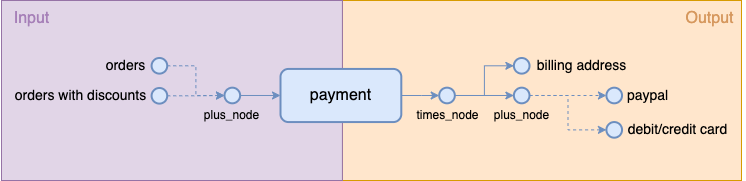
\includegraphics[width=\textwidth]{overleaf/images/template_example.png}
    \caption{Running Example}
    \label{fig:template_example}
\end{figure}

This example process in Figure \ref{fig:template_example} is an online payment process that computes an order with or without discounts coming in and asks the customer for the billing address and the payment method, which can be either PayPal or Debit/Credit card.

The order without discounts (\verb!order!) contains the order number (\verb!order id!) and the total price (\verb!total price!). The order with discounts contains the order number (\verb!order id!), the total price (\verb!total price!), and the discount percentage (\verb!discount!).
% additional to the order without discounts.
The billing address contains the home address (\verb!home address!) and country \verb!country! for the address in the receipt. The PayPal method only contains the PayPal account (\verb!account!). The Debit/Credit card contains the card number (\verb!card number!), the expired date (\verb!expired date!), and the security code (\verb!security code!).

% We will assume that \verb!orders!, being an entity, contains two fields: \verb!order id! and \verb!total price!; \verb!orders with discounts! contains three fields: \verb!order id!, \verb!total price!, and \verb!discount percent!; \verb!billing address! contains two fields: \verb!home address! and \verb!country!; \verb!paypal! contains only \verb!paypal account!; and \verb!debit/credit card! contains three fields: \verb!card number!, \verb!expire date!, and \verb!security code!.
